\documentclass{article}
\usepackage{tikz}
\usetikzlibrary{arrows}

\begin{document}

    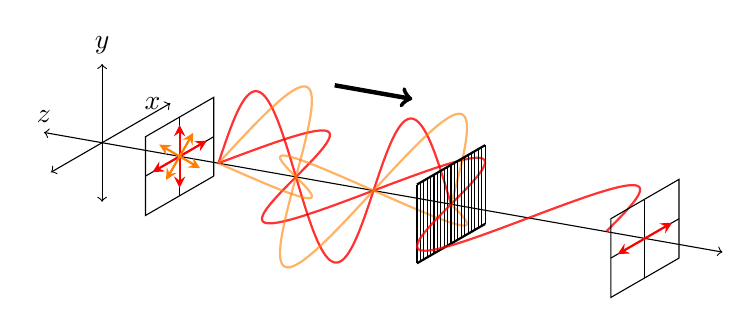
\begin{tikzpicture}[x={(-10:1cm)},y={(90:1cm)},z={(210:1cm)}]
        % Axes
        \draw[<->] (-0.75,0,0) node[above] {$z$} -- (8,0,0);
        \draw[<->] (0,-0.75,0) -- (0,1,0) node[above] {$y$};
        \draw[<->] (0,0,0.75) -- (0,0,-1) node[left] {$x$};

        % Unpolarized light
        \draw[red,thick,opacity=0.8] plot[domain=1.5:4.5,samples=200] (\x,{cos(deg(pi*\x))},0);
        \draw[red,thick,opacity=0.8] plot[domain=1.5:4.5,samples=200] (\x,0,-{cos(deg(pi*\x))});
        \draw[orange,thick,opacity=0.6] plot[domain=1.5:4.5,samples=200] (\x,{0.707*cos(deg(pi*\x))},-{0.707*cos(deg(pi*\x))});
        \draw[orange,thick,opacity=0.6] plot[domain=1.5:4.5,samples=200] (\x,{-0.707*cos(deg(pi*\x))},{-0.707*cos(deg(pi*\x))});
        
        % First pol. plane /w arrows
        \draw (1,-0.5,-0.5) -- (1,-0.5,0.5) -- (1,0.5,0.5) -- (1,0.5,-0.5) -- (1,-0.5,-0.5);
        \draw (1,0,-0.5) -- (1,0,0.5);
        \draw (1,-0.5,0) -- (1,0.5,0);
        
        \draw[<->, >=stealth, thick, red] (1,-0.4,0) -- (1,0.4,0);
        \draw[<->, >=stealth, thick, red] (1,0,-0.4) -- (1,0,0.4);
        \draw[<->, >=stealth, thick, orange] (1,-0.3,-0.3) -- (1,0.3,0.3);
        \draw[<->, >=stealth, thick, orange] (1,-0.2,0.2) -- (1,0.2,-0.2);
        
        % Wire grid
        \draw[thick] (4.5,0.5,0.5) -- (4.5,0.5,-0.5);
        \draw[thick] (4.5,-0.5,-0.5) -- (4.5,-0.5,0.5);
        \foreach \x in {-0.5,-0.45,...,0.55} {
          \draw[thin] (4.5,-0.5,\x) -- (4.5,0.5,\x);
        }
        
        % Polarized E-field
        \draw[red,thick,opacity=0.8] plot[domain=4.5:6.5,samples=200] (\x,0,-{cos(deg(pi*\x))});
        
        % Second pol. plane /w arrows
        \draw (7,-0.5,-0.5) -- (7,-0.5,0.5) -- (7,0.5,0.5) -- (7,0.5,-0.5) -- (7,-0.5,-0.5);
        \draw (7,0,-0.5) -- (7,0,0.5);
        \draw (7,-0.5,0) -- (7,0.5,0);
        
        \draw[<->, >=stealth, thick, red] (7,0,-0.4) -- (7,0,0.4);
        
        \draw[->,ultra thick] (3,1.25,0) -- node[above] {} (4,1.25,0);
        
    \end{tikzpicture}

\end{document}